\documentclass[a4paper,12pt]{article}
\usepackage{geometry}
\usepackage{fancyhdr}
%\renewcommand{\familydefault}{\sfdefault}
%\usepackage{fontenc}
%\usepackage{helvet}
%above 3 lines are the commands that implement Helvetica font
\usepackage{fontspec}
\setmainfont{Arial}
\usepackage{titlesec}
\titleformat*{\section}{\bfseries \normalsize}
\titleformat*{\subsection}{\bfseries \normalsize}
\titlelabel{\thetitle.\quad}
%the above 2 lines sets the section font as 12pt
\usepackage{parskip}
\usepackage{microtype}
\usepackage[british]{babel}
\usepackage{blindtext}
\usepackage{graphicx}
\usepackage{float}
%\usepackage[section]{placeins}
%line above prevents floating over sections
\usepackage{array}
%the array package enables options like >{}, <{} in the tabuler environment
\usepackage[font = footnotesize, justification = justified]{caption}
\usepackage{booktabs}
\setlength{\heavyrulewidth}{1.5pt}
\usepackage{siunitx}
\usepackage{url}
\begin{document}
{\pagestyle{empty}
	\begin{center}
		{\LARGE\bfseries An investigation into damping and resonance of a copper band\\
		
		}
		\vspace{\baselineskip}
		{\itshape 
		%Haoze Pang \\
		11019521\\
		}
		\vspace{\baselineskip}	
		Department of Physics and Astronomy\\
		The University of Manchester\\
		\vspace{\baselineskip}	
		First Year Laboratory Report\\
		\vspace{\baselineskip}	
		{\today}\\
		\vspace{2\baselineskip}		
		This experiment was performed in collaboration with 
		%\textit{Alec Bury 10833524}.
	\end{center}
	\vspace{4\baselineskip}
	\textbf{Abstract}
	
	In this experiment, we investigated the effect of damping and resonance of a copper band. The experiment was divided into two parts. In the first part, we created harmonic oscillatory environment, focusing on damping, which we characterised by quality factor \( Q \). We performed three trials in this part of the experiment, varying the damping parameter from the Helmholtz coils. The quality factor was calculated to be \( 253.5587 \pm 0.0005 \) for the first trial without damping from the coils, \(229.0207 \pm 0.0005 \) for a damping parameter of 100, \( 186.8327 \pm 0.000 \) for a damping parameter of 225. In the second part of the experiment, we applied a driving force to investigate the effect of resonance. The resonance frequency of the copper band \( f_0 \) was determined to be \( 17.0000 \pm 0.0025 \unit{\per\second} \).  
\clearpage}
\section{Introduction}
Oscillatory systems are ubiquitous, from the mechanical mass-spring system, to LCR circuits, to chemical bonds. The study of oscillatory system is therefore important.  A typical oscillatory system possess a variety of qualities, but damping and resonance \cite{resonancescience} are perhaps the most obvious one. Their application in reducing frictions and avoiding unwanted oscillation is essential. Therefore, we conducted an experiment to investigate the effect of damping and resonance.
\section{Theory}
\subsection{Damped harmonic oscillation}
The presence of a damping force whose magnitude is proportional to the speed of oscillation is the defining characteristic of damped oscillation\cite[Chapter~14]{Young&Freedman}. In damped harmonic oscillation, the governing equation:
\begin{equation}
	\label{eqn: damped ge}
	m\frac{d^2x}{dt^2}+b\frac{dx}{dt}+kx=0
\end{equation}
can be derived from N2. In this equation, \( m \) stands for the mass of the object, \( b \) for the  proportionality constant of the damping force, \( k \) the proportionality constant of the restoring force, and \( x \) the displacement from equilibrium position.
Solving this ODE, we obtain the position equation:
\begin{equation}
	\label{eqn: damped sln}
	x(t) = A_0e^{-\frac{\gamma}{2}t}\cos(\omega_0 t + \phi),
\end{equation}
where \( \gamma = \frac{b}{m} \) is referred to as the damping factor and  \( \omega_0^2 = \frac{k}{m} \) the natural frequency. For all harmonic oscillation parts in this report, we denote \( A_h \equiv A_h(t) = A_0e^{-\frac{\gamma}{2}t} \), as the amplitudes.

The quality factor is defined as \( Q = \frac{\omega_0}{\gamma} \). This factor reflects the effect of damping on the system. The greater the damping, the lower the value of quality factor. 
\subsection{Forced oscillation}
Forced oscillations \cite[Chapter~4]{King} occur when a driving force is applied. In such case, the RHS of equation \ref{eqn: damped ge} becomes the driving force, i.e.
\begin{equation}
	\label{eqn: forced ge}
	m\frac{d^2x}{dt^2}+b\frac{dx}{dt}+kx = F_0\cos(\omega t).
\end{equation}
Notice that the complimentary function of the solution to equation \ref{eqn: forced ge} corresponds to the system's transient response. Solving for the particular integral, we obtained the amplitude of forced oscillation:
\begin{equation}
	A = \frac{F_0/m}{\sqrt{(\omega_0^2 - \omega^2)^2 + \gamma^2 \omega_0^2}}.
\end{equation}

The average power over one period of oscillation can be shown to be
\begin{equation}
	\label{eqn: avg p}
	\overline{P}(\omega) = \frac{1}{2}bv_0^2 = \frac{1}{2}\frac{F_0^2\omega^2 \gamma^2}{m(\omega_0^2 - \omega^2)^2 + (\omega\gamma)^2},
\end{equation}
where \( v_0 = A\omega \). Notice that \( \overline{P}_{max} \) occurs at \( \omega = \omega_0 \).
If we define \( \Delta \omega = \omega - \omega_0 \),  we can see that \( \frac{1}{2} \overline{P}_{max} \) happens when \( \frac{2\Delta \omega}{\gamma} = 1\). Therefore, the full width at half maximum \( \omega_{fwhm} = 2\Delta \omega\) can be expressed as
\begin{equation}
	\omega_{fwhm} = \gamma.
\end{equation}
This result is particularly useful since we can use the plot of \( \overline{P}(\omega) \) to determine the damping factor.
\section{Experimental Method}
\subsection{Experiment setup}
The experiment was set up  as follows. A copper band was clamped at its right end and placed horizontally. The left end of the copper band was able to move freely, and was placed between two Helmholtz coils. Right to the Helmholtz coils, another coil was wrapped around the copper band and is place in the concave of a horseshoe magnet. Right to the coils a loudspeaker was placed below the copper band. The loudspeaker had a removable rubber band which can be attached to the copper band, producing a driven frequency.
\begin{figure}[h]
	\centering
	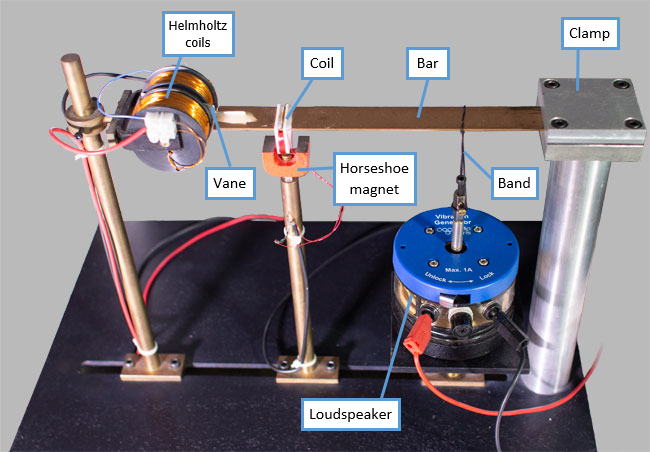
\includegraphics[scale=0.4]{Images/IMG_1805_equipment-labelled.jpg}
	\caption{This figure \cite{Prelab} shows experiment setup.}
\end{figure}

A function generator was linked to the loudspeaker, and a digital oscilloscope was connected to the  coil wrapping the copper band. Throughout the experiment, the function generator was used to generate certain driving frequency and the oscilloscope was employed to read the velocity of the copper band. A signal amplifier was connected to both devices and was also linked to the Helmholtz coil to introduce extra damping in the system.
\begin{figure}[h]
	\centering
	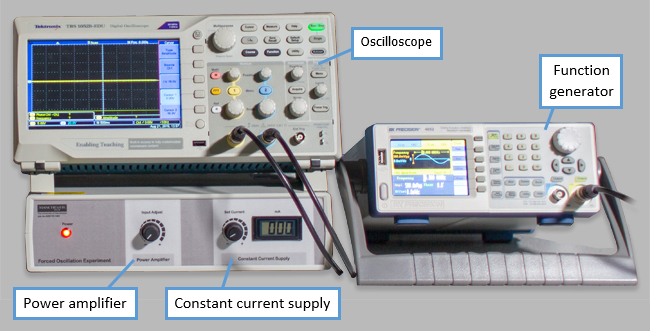
\includegraphics[scale=0.4]{Images/Equipment-scopes-and-power-labelled.jpg}
	\caption{This figure \cite{Prelab} the oscilloscope and function generator used in the experiment.}
\end{figure} 
\subsection{Damped harmonic oscillation}
The rubber band was removed from the copper band, and damping from Helmholtz coils was set to \( 0 \). The experimenter plugged the left end of the copper band to cause it to vibrate. He then recorded the speed of the copper band as a function of time in an Excel document. Two similar trials was conducted, setting the damping parameter in the Helmholtz coils to be 100 and 225. 
\subsection{Forced oscillation}
After collecting all three sets of data from the first part of this experiment, the rubber band was attached to the copper band. In the first trial of forced oscillation, the damping from the Helmholtz coils was turned to  \(0 \). Function generator was used to produce varying driving frequencies. The experimenter then read \( v_0 \) from the oscilloscope. Two additional trials were conducted with the same procedure, but setting the damping parameter from the coils to be 100 and 225.
\section{Data and analysis}
\subsection{Damped harmonic oscillation}
Notice that equation \ref{eqn: damped sln} implies a method to determine \( \gamma \) from maximum amplitude. Specifically, the gradient of the plot \( -2\ln A_h \) against time, \( t \), is \( \gamma \). For each of the 3 trials, the experimenter selected the amplitudes from the dataset, and then  plotted \( -2\ln A_h \) against time (by least square regression, LSFR), and determined the corresponding \( \gamma \) from the slope. During the LSFR process, the dominant source of error was decided to be \( -2\ln A_h \). Specifically, the error on the dependent variable was \( 0.01 \) for all \( t \), which came from the resolution of the oscilloscope. To calculate the quality factor, we found the average period \( T \) of the oscillation by subtracting the time between two consecutive amplitudes, and averaging of result. 

Now, we present the result from the three trials.
\begin{figure}[h]
	\centering
	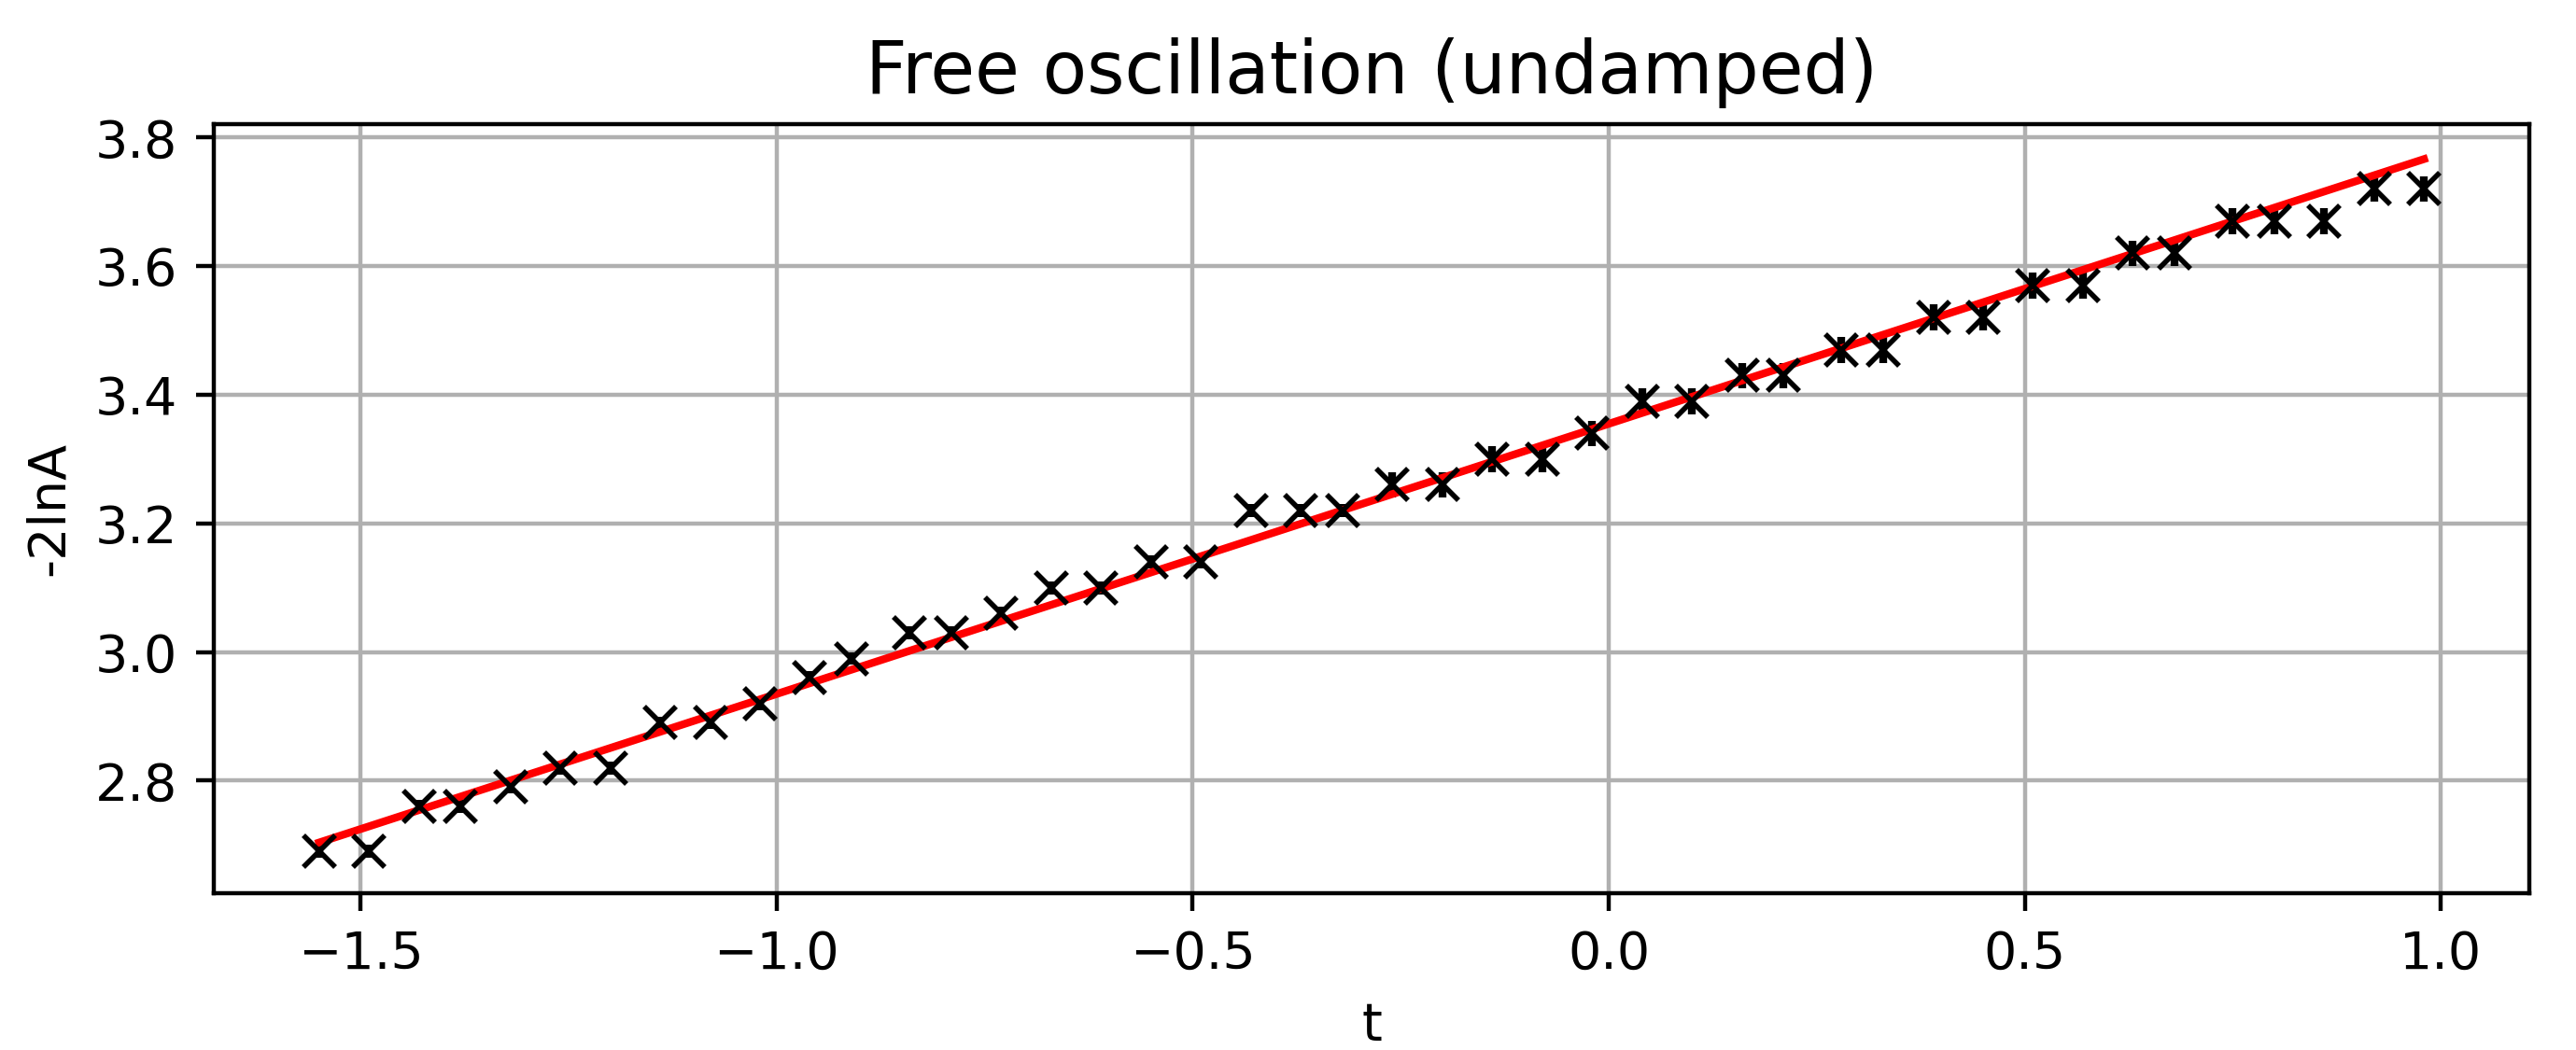
\includegraphics[scale=0.5]{images/free_undamped_LSFR.png}
	\caption{This is the LSFR fit for the harmonic oscillation without extra damping from the Helmholtz coils.}
\end{figure}
For the first trial (without extra damping from Helmholtz coils), the slope of the from the LSFR was \( \gamma = \num{4.20d-1} \pm \num{3d-3} \unit{\per\second} \), with reduced \( \chi^2 = 2.51 \). We determined \( T = 0.0588 \pm 0.0001 \unit{\second} \). Therefore,
\begin{equation}
	Q_{h1} = \frac{2\pi}{\gamma T} = 253.5587 \pm 0.0005.
\end{equation} 
\begin{figure}[h]
	\centering
	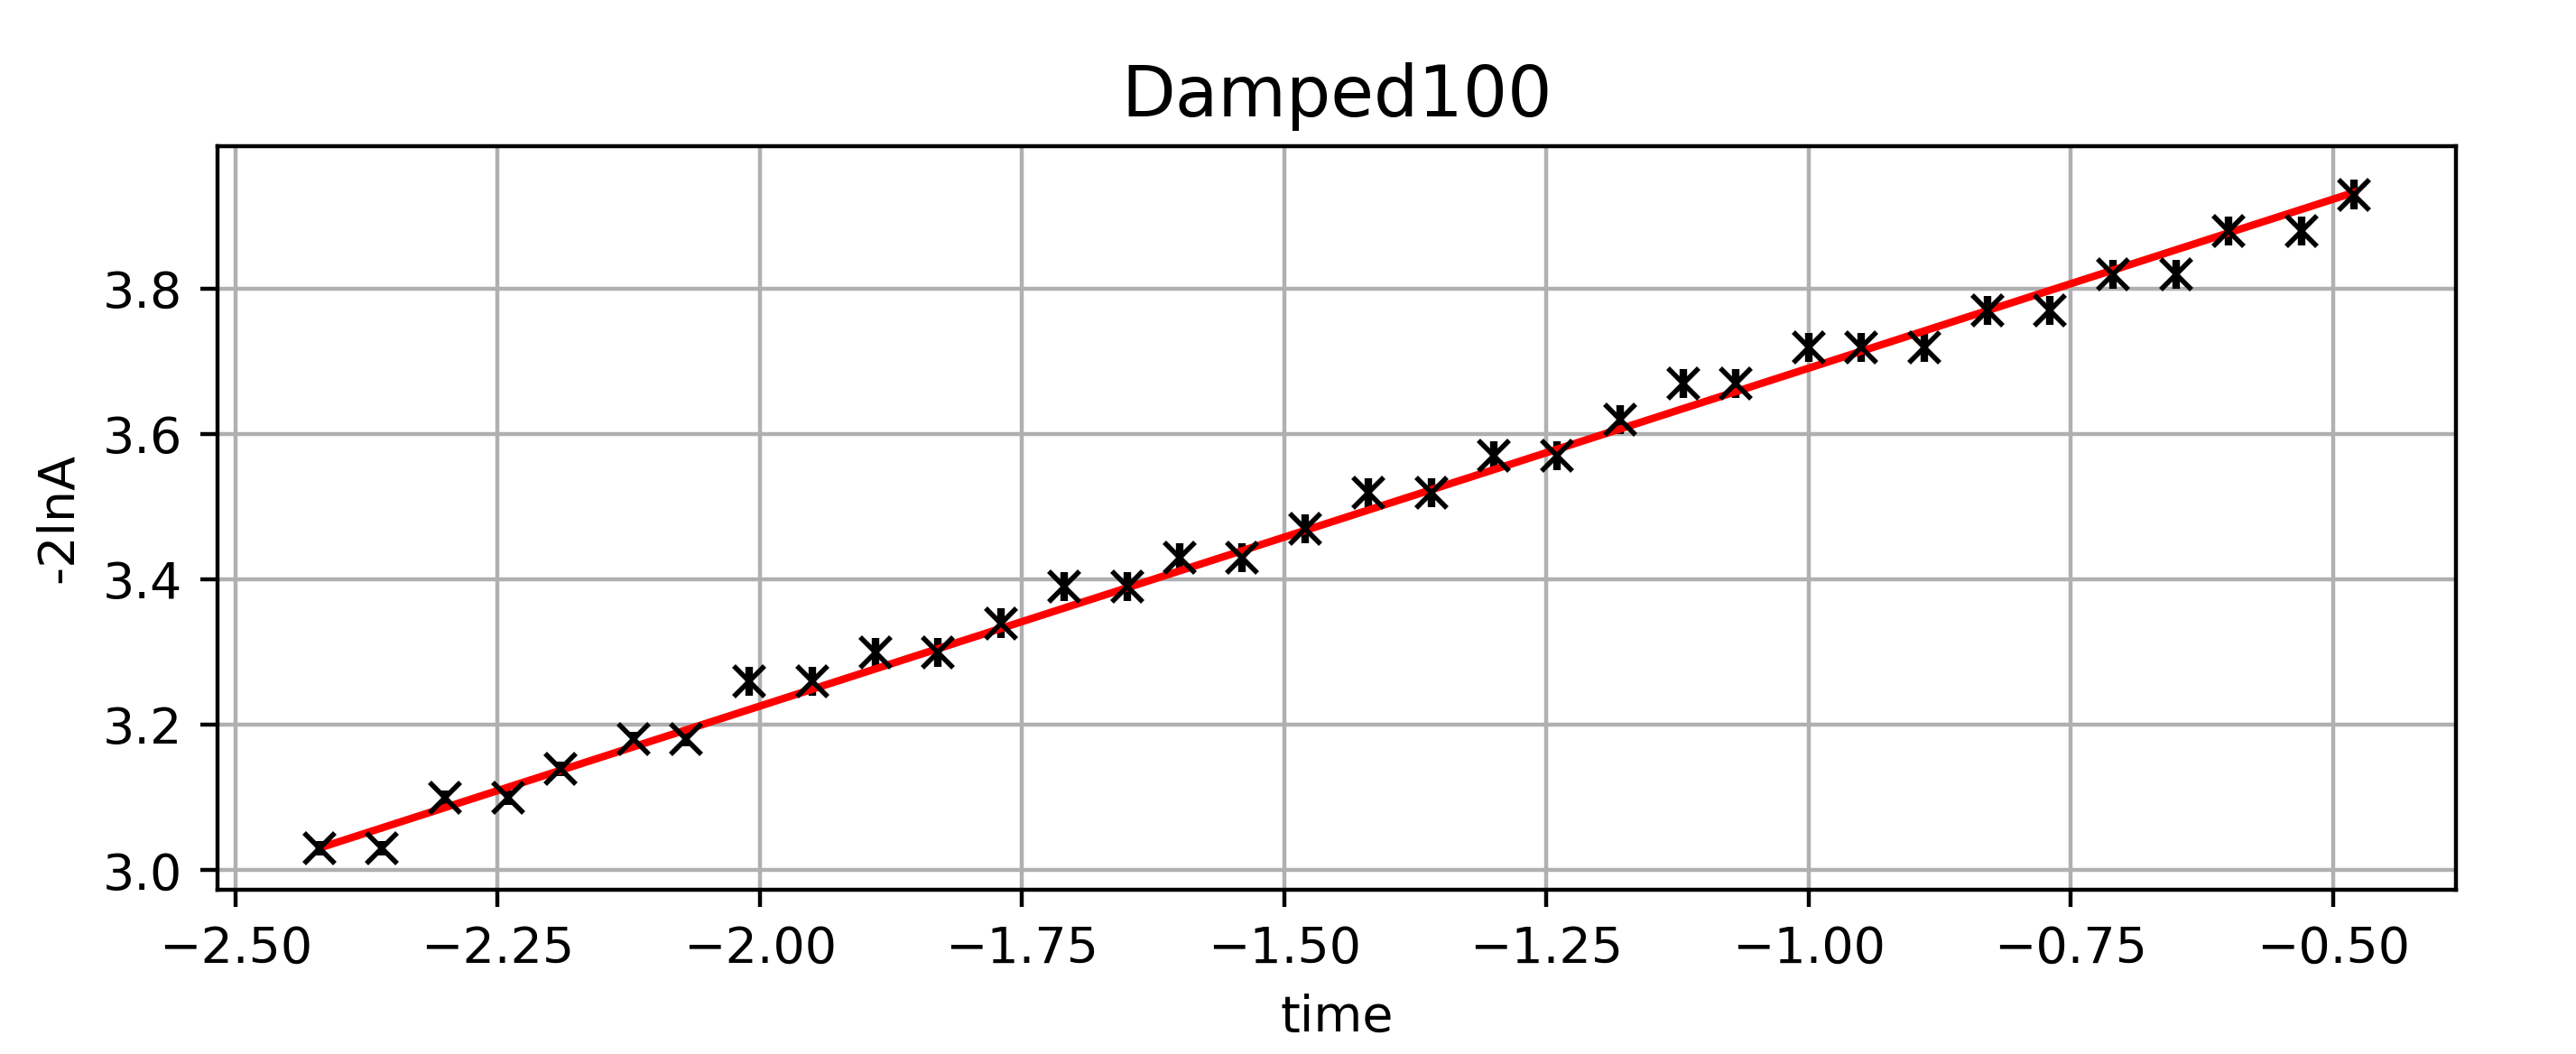
\includegraphics[scale=0.5]{images/damped100.png}
	\caption{This is the plot for the harmonic oscillation with damping parameter of 100.}
\end{figure}
In the second trial (with damping parameter of 100), the slope of the from the LSFR was \( \gamma = \num{4.65d-1} \pm \num{4d-3} \unit{\per\second} \), with reduced \( \chi^2 = 1.27 \). We determined \( T = 0.0587 \pm 0.0001 \unit{\second} \). Therefore,
\begin{equation}
	Q_{h2} = \frac{2\pi}{\gamma T} = 229.0207 \pm 0.0005.
\end{equation} 
\begin{figure}[h]
	\centering
	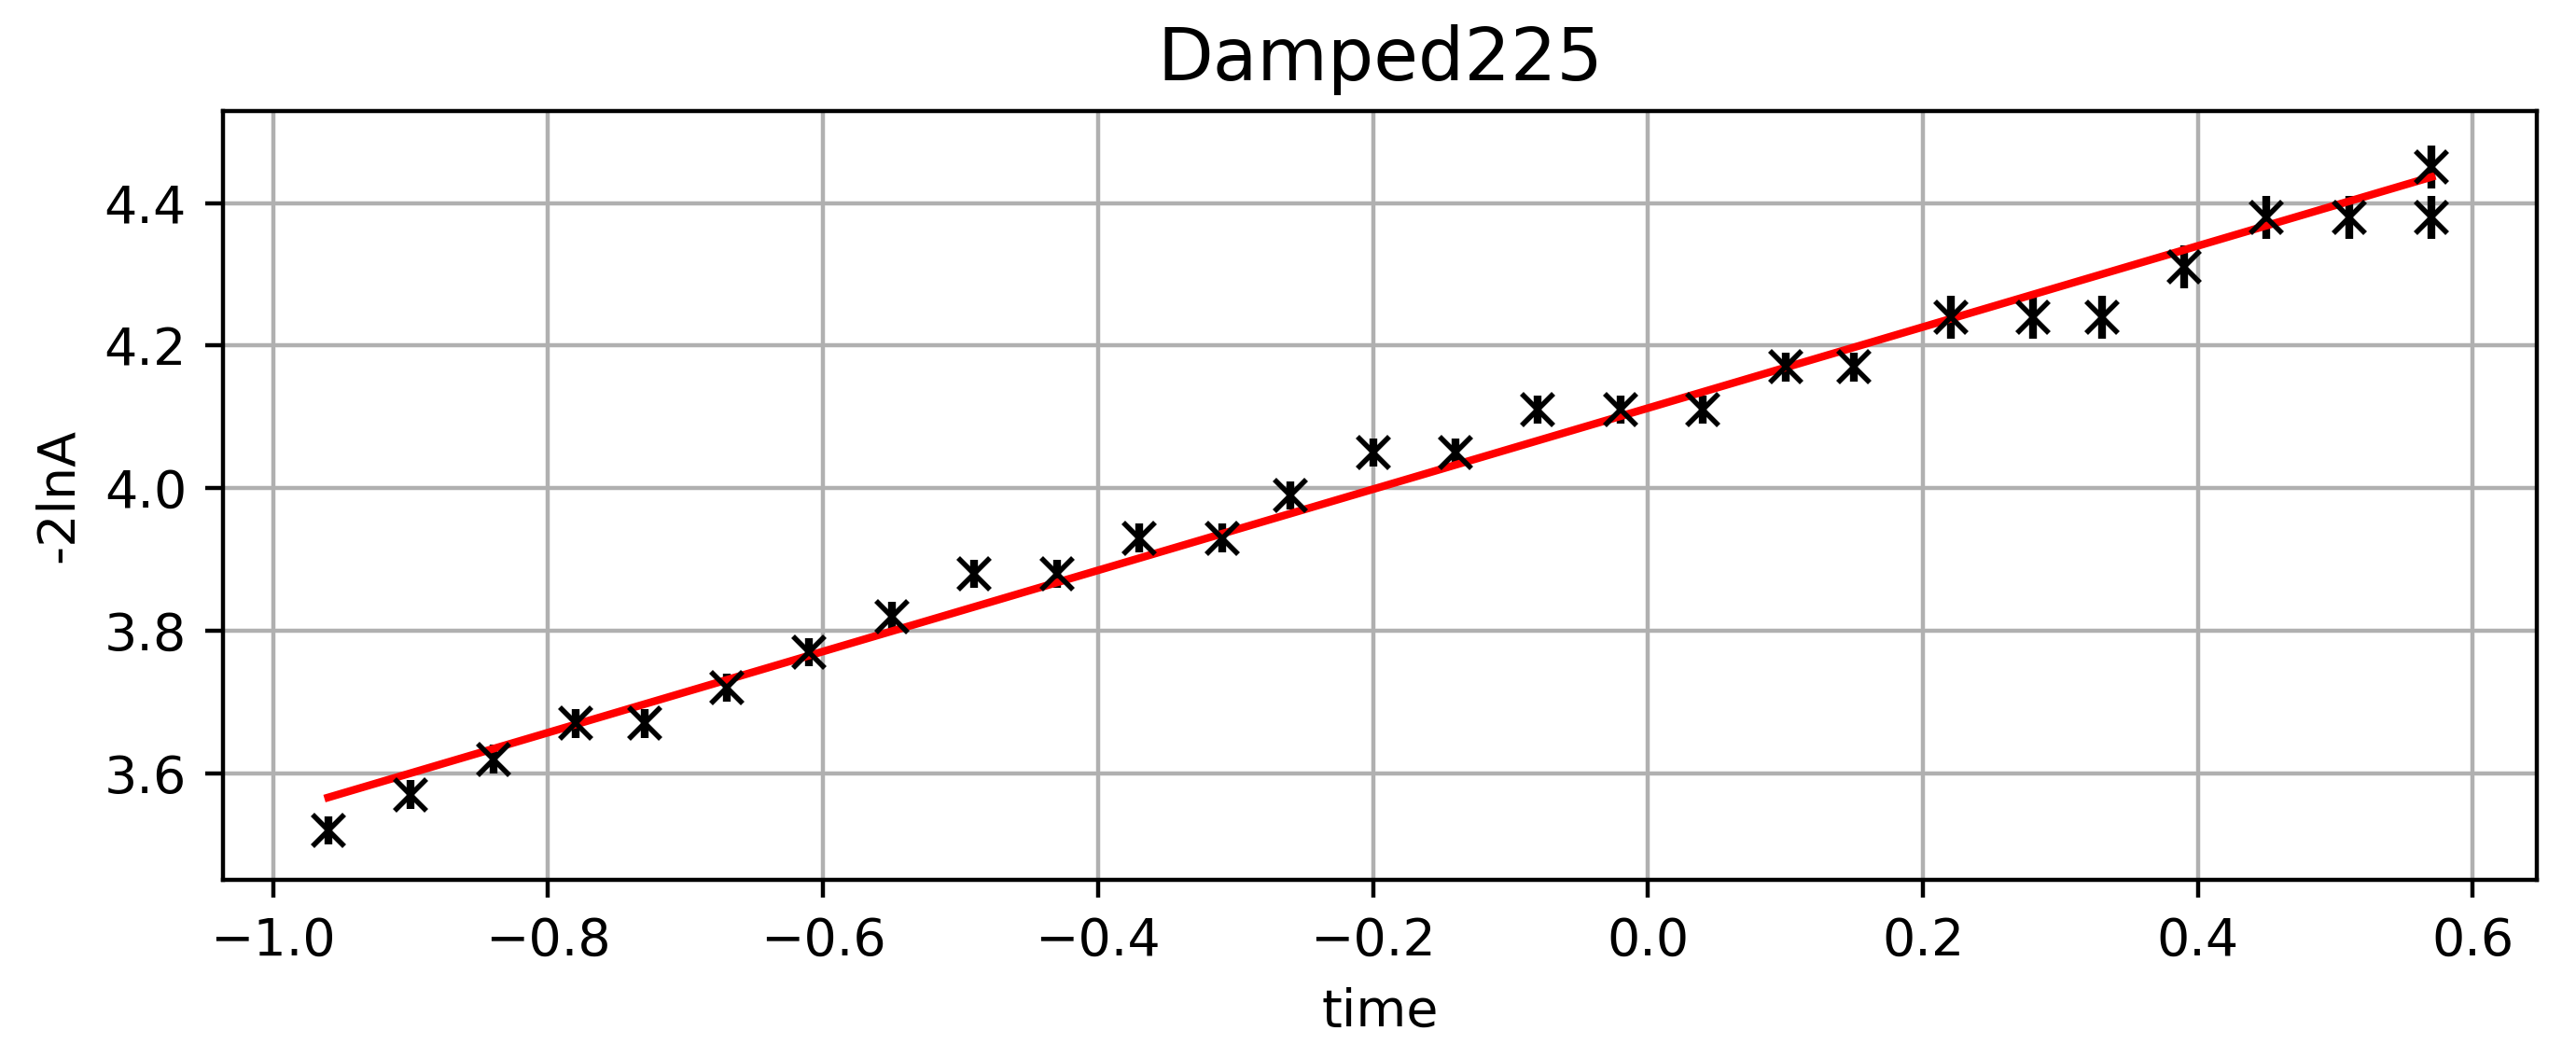
\includegraphics[scale=0.5]{images/damped225.png}
	\caption{This is the plot for the harmonic oscillation with damping parameter of 225.}
\end{figure}
For the third trial (with damping parameter of 225), the slope of the from the regression was \( \gamma = \num{5.7d-1} \pm \num{1d-2} \unit{\per\second} \), with reduced \( \chi^2 = 1.80 \). We determined \( T = 0.0588 \pm 0.0001 \unit{\second} \). Therefore,
\begin{equation}
	Q_{h3} = \frac{2\pi}{\gamma T} = 186.8327 \pm 0.0008.
\end{equation} 
\subsection{Forced oscillation}
In the first trial, using Origin Lab, the experimenter used Gaussian fit to plot \( v_0^2 \) against the driving frequency \( f \). 
\begin{figure}[h]
	\centering
	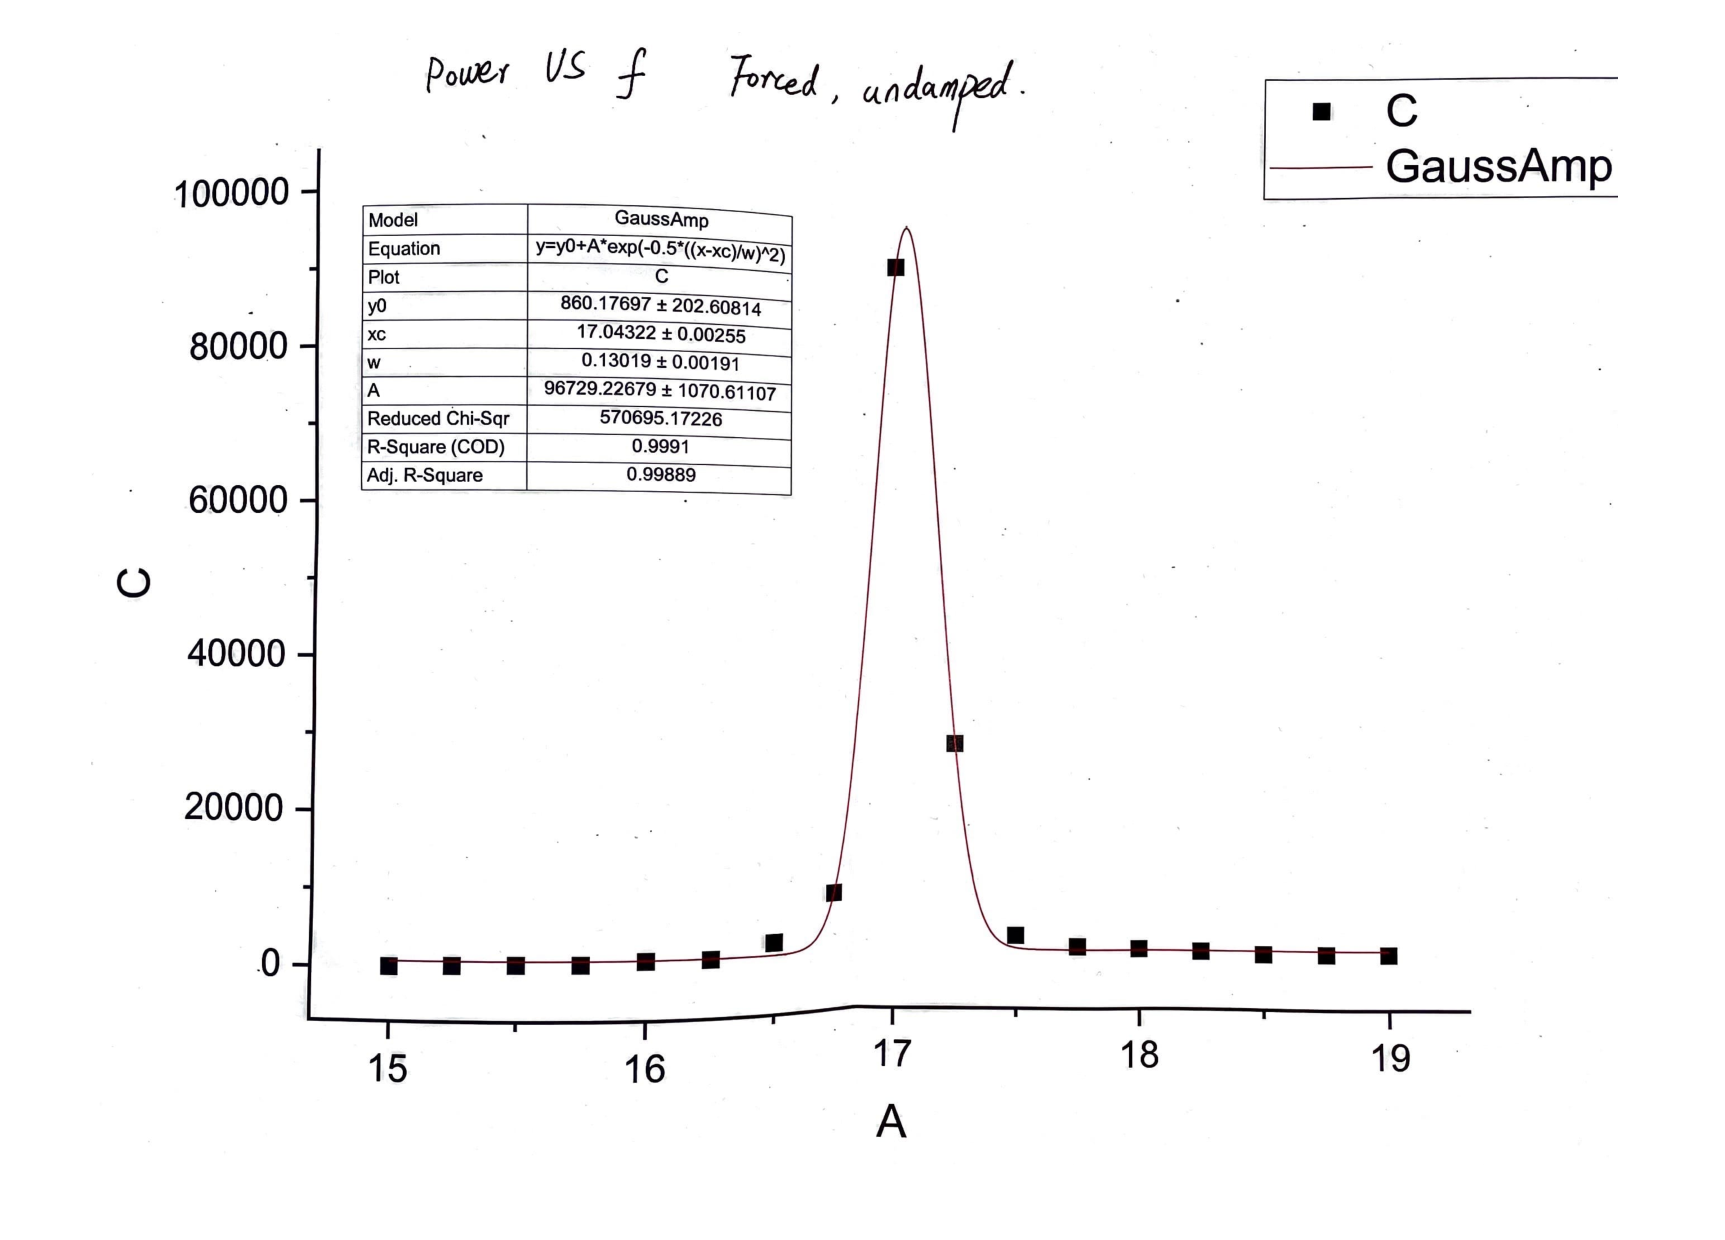
\includegraphics[scale=0.4]{images/undamped.pdf}
	\caption{This is a Gaussian fit for \(v_0^2 \) against \( f \) from forced oscillation without extra damping from the Helmholtz coils.}
\end{figure}
From this Gaussian fit analysis, we knew \(\omega_{fwhm} = \gamma = 0.307 \pm 0.005 \unit{\per \second} \) and \( f_0 = 17.0000 \pm 0.0025 \unit{\per\second} \). Therefore, the quality factor was given by
\begin{equation}
	Q_1 = \frac{2\pi f}{\gamma} = 348 \pm 6.
\end{equation}
In the second trial, using Origin Lab, the experimenter used Gaussian fit to plot \( v_0^2 \) against the driving frequency \( f \). 
\begin{figure}[h]
	\centering
	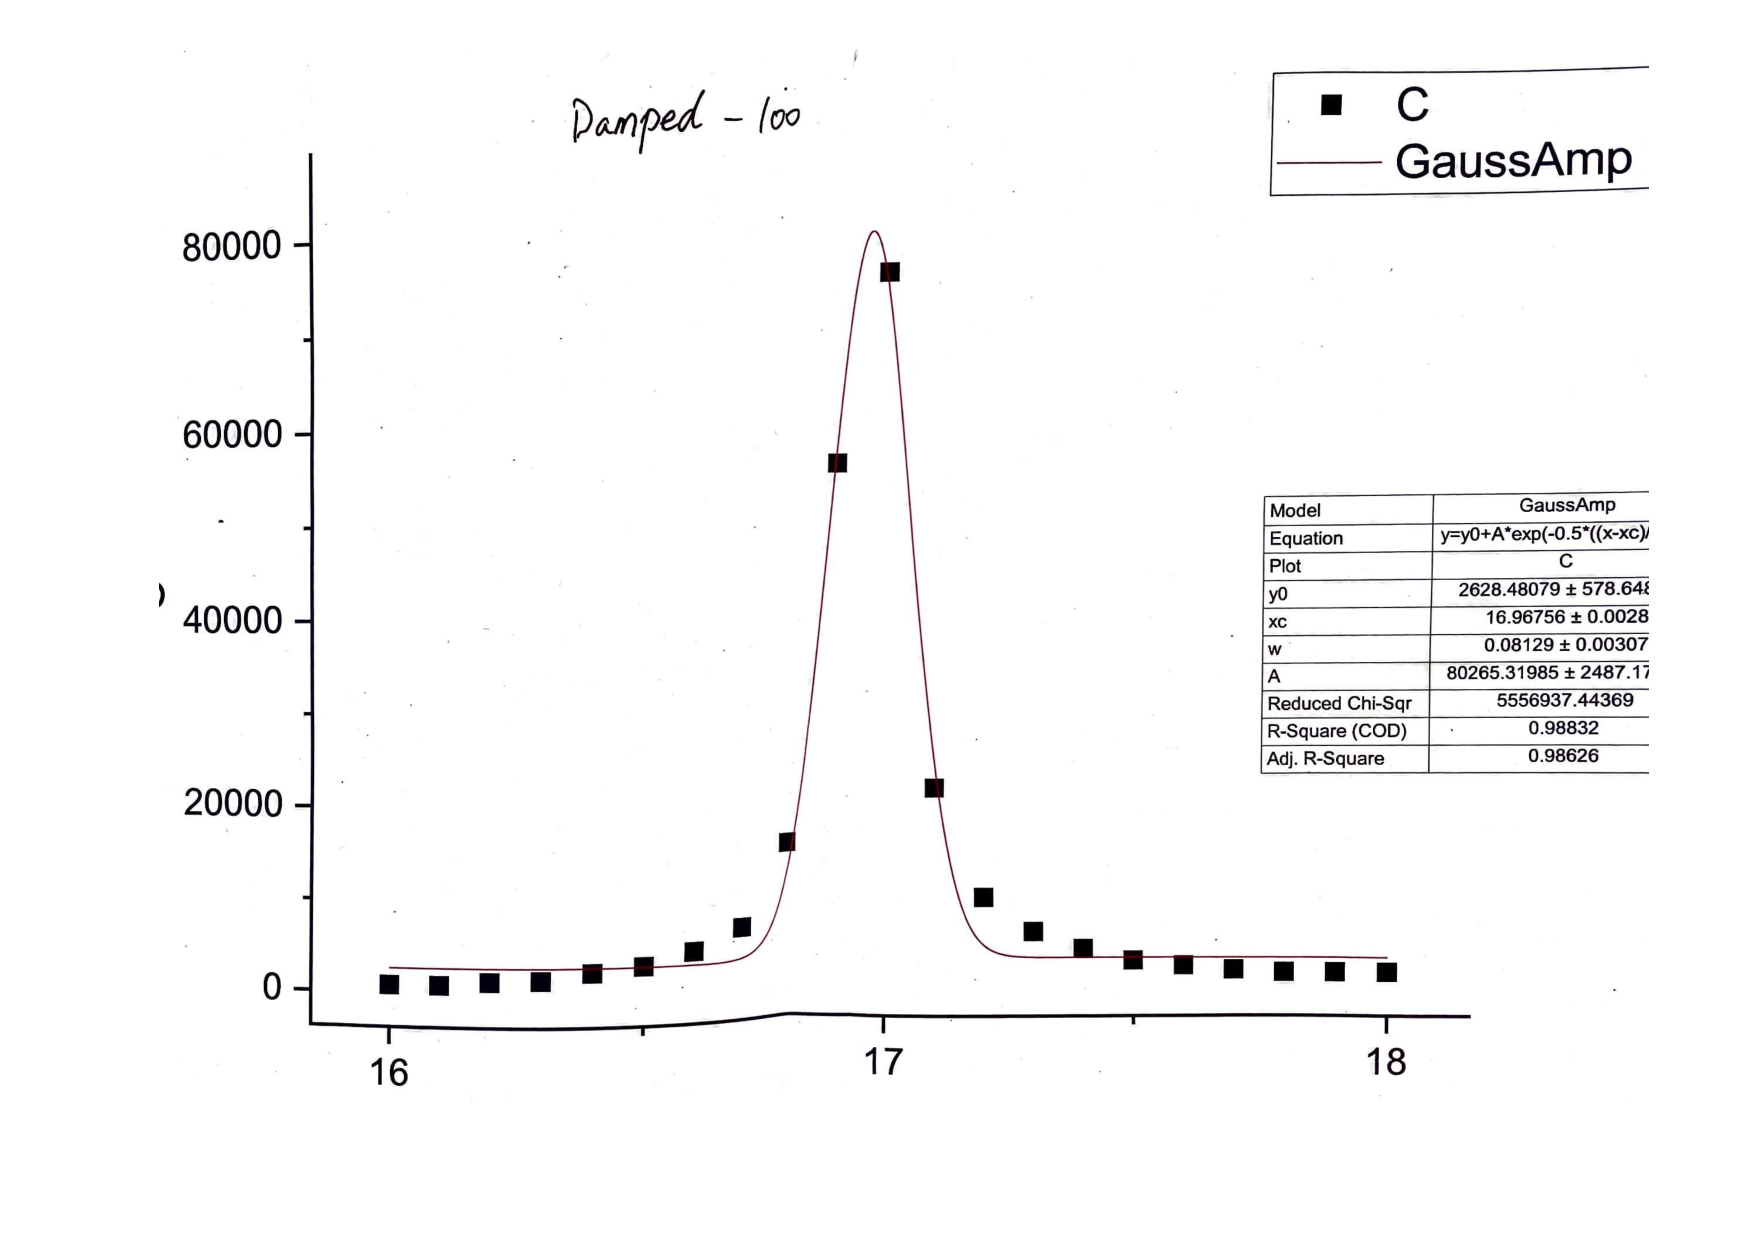
\includegraphics[scale=0.4]{images/damped100.pdf}
	\caption{This is a Gaussian fit for \(v_0^2 \) against \( f \) for the forced oscillation with extra damping parameter of 100 from the Helmholtz coils.}
\end{figure}
From this Gaussian fit analysis, we knew \(\omega_{fwhm} = \gamma = 0.191 \pm 0.007 \unit{\per \second} \) and \( f_0 = 16.9676 \pm 0.0028 \unit{\per\second} \). Therefore, the quality factor was calculated to be
\begin{equation}
	Q_2 = \frac{2\pi f}{\gamma} = 558 \pm 20.
\end{equation}
In the third trial, using Origin Lab, the experimenter fitted a Gaussian plot for \( v_0^2 \) against \( f \). 
\begin{figure}[h]
	\centering
	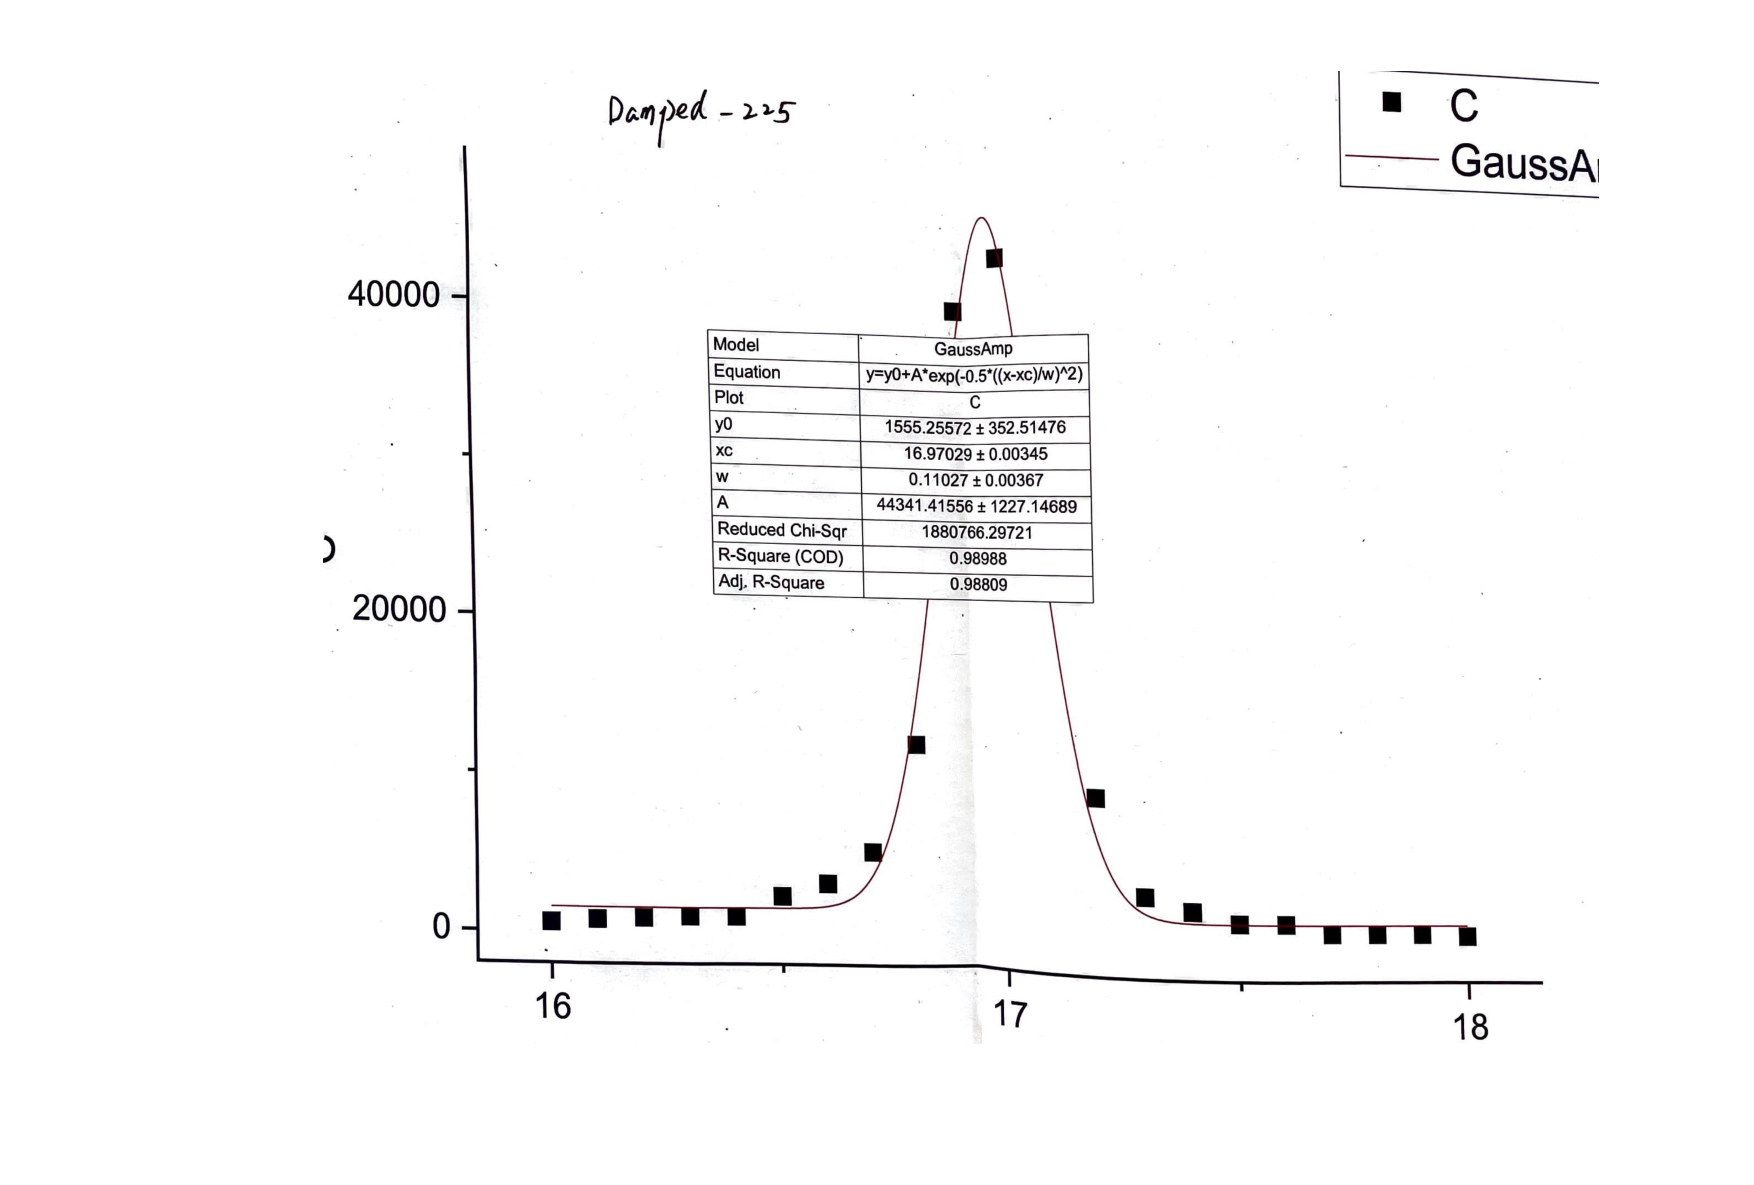
\includegraphics[scale=0.4]{images/damped225.pdf}
	\caption{This is a Gaussian fit for \(v_0^2 \) against \( f \)   for the forced oscillation with extra damping parameter of 100 from the Helmholtz coils.}
\end{figure}
From this Gaussian fit analysis, we knew \(\omega_{fwhm} = \gamma = 0.260 \pm 0.009 \unit{\per \second} \) and \( f_0 = 16.97029 \pm 0.00345 \unit{\per\second}\). Therefore, the quality factor is given by
\begin{equation}
	Q_3 = \frac{2\pi f}{\gamma} = 410 \pm 14.
\end{equation}
\clearpage
\section{Results and discussion}
\subsection{Harmonic oscillation}
We summarised the result from the first part of our experiment in table \ref{tbl:harmoni}.
\begin{table}
	\centering
	\begin{tabular}{*{2}{>{\(}c<{\)}}}
		\toprule
		\text{Extra damping from the Helmholtz coils}  & \text{Quality factor}\\
		\cmidrule(lr){1-1} \cmidrule(lr){2-2}  
		0 & 253.5587 \pm 0.0005\\
		100 & 229.0207 \pm 0.0005\\
		225 & 186.8327 \pm 0.0008\\
		\bottomrule
	\end{tabular}
	\caption{Summary of results from harmonic oscillation.}
	\label{tbl:harmoni}
\end{table}
These results are consistent with the property of quality factor. That is, the greater the damping, the smaller the \( Q \) value. Theses results are also very precise. The uncertainties are small.  As for the LSFR process, the graph is a good fit for the data judging from small values of reduced \( \chi^2 \).
\subsection{Forced oscillation}
We summarised the result from the forced oscillation part in table \ref{tbl:forced}.
\begin{table}
	\centering
	\begin{tabular}{*{3}{>{\(}c<{\)}}}
		\toprule
		\text{Extra damping from the Helmholtz coils}  & \text{Quality factor} & \text{resonance freqency}\\
		\cmidrule(lr){1-1} \cmidrule(lr){2-2}  \cmidrule(lr){3-3}
		0 & 348 \pm 6 & 17.0000 \pm 0.0025 \unit{\per\second}\\
		100 & 558 \pm 20 & 16.9676 \pm 0.0028 \unit{\per\second}\\
		225 & 410 \pm 14 & 16.97029 \pm 0.00345 \unit{\per\second}\\
		\bottomrule
	\end{tabular}
	\caption{Summary of results from forced oscillation.} 
	\label{tbl:forced}
\end{table}
Notice for the force oscillation, the result is inconsistent with the property of quality factor. This may be due to the error in the analysis process. In the forced oscillation part of the experiment, we used Gaussian fit to find \( \omega_{fwhm} \), but the better method is Lorentzian fit. The resonance frequency is fairly consistent (about \( 17 \unit{\per\second} \) ).
\section{Summary}
We have investigated the effect of damping and resonance of oscillation. Specifically, we characterised damping with quality factor \( Q \). We divided this experiment into two parts. in the first part, we focused on the effect of damping, in the second part, resonance. The results are generally consistent with the expectation. However, due to a data analysis error, we obtained bizarre figures for the quality factor in the second part of the experiment. Suggestions are made on how to improve the analysis method for more accurate results.   
\bibliographystyle{plain}
\bibliography{Undergraduate-lab-report-common-references.bib}
\end{document}